\documentclass[letter,11pt]{article}
%\documentclass[letter,twoside,11pt]{article}

\usepackage[spanish,es-nodecimaldot]{babel}
\usepackage[utf8]{inputenc}

\usepackage{lmodern}
\usepackage[T1]{fontenc}
\usepackage{textcomp}

\usepackage{graphicx}
\usepackage{pstricks}

\usepackage{anysize}
\marginsize{3cm}{2cm}{2cm}{3cm}

\usepackage{amsmath}
\usepackage{array}
\usepackage{gensymb}
\usepackage{alltt}

\usepackage{fancyhdr}
\usepackage{lastpage}
\pagestyle{fancy}
\fancyhf{}
\fancyhead[LE,RO]{Laboratorio de Física Básica I}
\fancyfoot[CO,CE]{\thepage\ de \pageref{LastPage}}

\special{papersize=215.9mm,279.4mm}

\usepackage[
    pdfauthor={Carlos Eduardo Caballero Burgoa},%
    pdftitle={Laboratorio de Física Básica I},%
    pdfsubject={Gráficas y ecuaciones},%
    colorlinks,%
    citecolor=black,%
    filecolor=black,%
    linkcolor=black,%
    urlcolor=black,
    breaklinks]{hyperref}
\usepackage{breakurl}

\newcommand{\blankpage}{
\newpage
\thispagestyle{empty}
\mbox{}
\newpage
}

\renewcommand{\arraystretch}{1.2}

\begin{document}

\begin{titlepage}
\begin{center}
{\Large UNIVERSIDAD MAYOR DE SAN SIMÓN}\\
\vspace*{0.15cm}
{\large FACULTAD DE CIENCIAS Y TECNOLOGÍA}\\
\vspace*{0.10cm}
DEPARTAMENTO DE FÍSICA\\
\vspace*{3.0cm}
{\Large \textbf{LABORATORIO DE FÍSICA BÁSICA I}}\\
\vspace*{0.3cm}
{\Large \textbf{PRACTICA No. 3}}\\
\vspace*{3.5cm}
{\Large \textbf{GRÁFICAS Y ECUACIONES}}\\
\end{center}

\vspace*{7.4cm}
\leftskip=7.95cm
\noindent
\textbf{Estudiante:}\\
Caballero Burgoa, Carlos Eduardo.\\
\newline
\textbf{Docente:}\\
Msc. Guzmán Saavedra, Rocio.\\
\newline
\textbf{Grupo:} N5.\\
\textbf{Fecha de realización:} 19 de Octubre del 2020.\\
\textbf{Fecha de entrega:} 20 de Octubre del 2020.\\

\end{titlepage}

\blankpage

\section{Objetivo}
Desarrollar la destreza de los alumnos en la graficación de datos y la obtención
por métodos gráficos de la relación entre las variables.

\section{Marco teórico}
En física experimental es común trabajar con dos variables, una llamada variable
independiente ($X_i$) que puede ser controlada, y la otra llamada variable
dependiente ($Y_i$). Ante los cambios de $X_i$, el sistema revela el
comportamiento a través de los cambios de sufre la variable $Y_i$.

Un gráfico es una adecuada representación gráfica de los datos experimentales en
un sistema de ejes perpendiculares, esta relación visual puede describirse a
través de una ecuación conocida como relación funcional entre ambas variables.

Por convención la variable independiente es la magnitud cuyo valor se escoge
cada vez, se representa en el eje horizontal, y la variable dependiente es el
valor que se determina, se representa en el eje vertical.

Existen dos tipos de escalas: las escalas lineales son aquellas en las que
distancias iguales representan cantidades iguales; las escalas no lineales son
aquellas que se construyen en base a un patrón de comportamiento que hace que
distancias iguales no representen cantidades iguales.

\subsection{Relación lineal}
En una gráfica lineal la linea que representa este comportamiento se trazara de
modo que pase por la mayoría de los puntos, o de tal forma que estos estén
distribuidos a ambos lados de la recta.

El modelo matemático para un comportamiento lineal es la ecuación de la linea
recta y la forma general es:

\begin{equation}
    y = A + B x
\end{equation}

Donde $A$ es la ordenada al origen y representa el valor de $y$ cuando $x = 0$,
su valor se lee en el punto de intersección de la recta con el eje de
coordenadas.

$B$ es la pendiente de la recta y se calcula mediante el cociente
$\Delta y/\Delta x$, donde $\Delta y$ es la diferencia de ordenadas y $\Delta x$
es la diferencia de abscisas, de dos puntos cualesquiera que estén sobre la recta
y representa el valor de la rapidez con que cambia $y$ respecto a $x$.

\subsection{Relación no lineal}
Cuando en la representación de datos experimentales en coordenadas rectangulares
no se obtienen lineas rectas, no es posible determinar directamente la relación
funcional entre las variables que interactúan, entonces se busca un método
(linealización) mediante el cual la relación entre los datos se convierta en una
relación lineal, de la cual es fácil determinar su ecuación y partir de la misma
obtener la relación funcional entre las variables originales (ecuación de la
curva).

Este método consiste básicamente en asumir un modelo para el comportamiento de
los datos, realizando un cambio de variable o aplicando logaritmos al modelo, la
nueva gráfica sera lineal si el modelo es el adecuado, caso contrario la gráfica
no sera lineal.

\section{Materiales}
\begin{itemize}
\item Luxómetro.
\item Flexometro.
\item Simulador «bajo presión 1.1.18».
\item Simulador «Lab de Péndulo».
\end{itemize}

\section{Procedimiento}
A continuación se describen los procedimientos experimentales que se llevarán a
cabo.

\subsection{Intensidad lumínica}
\begin{enumerate}
\item Armar un trípode para establecer una posición fija para la medición.
\item Establecer una fuente lumínica con intensidad moderada.
\item Medir la intensidad lumínica lo mas próximo a la fuente como sea posible.
\item Repetir la medición para diferentes distancias de la fuente hasta 20
veces.
\end{enumerate}

\subsection{Presión vs profundidad}
\begin{enumerate}
\item Iniciar el simulador de presión.
\item Llenar el tanque de agua.
\item Posicionar una regla para la medición de profundidad.
\item Con el sensor de presión, medir la presión a 0 metros de profundidad.
\item Repetir la medición por cada unidad mínima de la regla hasta 15 veces.
\end{enumerate}

\subsection{Resistencia vs temperatura}
\begin{enumerate}
\item A partir de los datos provistos en la tabla, realizar la graficación,
y el calculo de la ecuación de su gráfica.
\end{enumerate}

\subsection{Péndulo}
\begin{enumerate}
\item Iniciar el simulador de péndulo simple.
\item Fijar un cronometro en el simulador.
\item Establecer una masa fija para el experimento.
\item Para cada variación de la longitud del péndulo, medir el tiempo de una
oscilación que no exceda los 10° de inclinación inicial.
\item Repetir la medición anterior hasta 30 veces.
\end{enumerate}

\section{Tablas de datos y resultados}

\subsection{Intensidad lumínica}

\begin{description}
\item[Instrumento utilizado:] Luxómetro.
\item[Precisión del instrumento:] $1 [lx]$
\item[Instrumento utilizado:] Flexometro.
\item[Precisión del instrumento:] $0.01 [m]$
\end{description}

\subsubsection{Datos obtenidos}

\begin{center}
\begin{tabular}{|c|>{\centering}m{2.8cm}<{\centering}
                  |>{\centering}m{2.8cm}<{\centering}|}
\hline
$i$ & $x_i[m]$ & $I_i[lux]$ \tabularnewline \hline
  1 & 0.00 & 300 \tabularnewline \hline
  2 & 0.20 & 287 \tabularnewline \hline
  3 & 0.30 & 230 \tabularnewline \hline
  4 & 0.42 & 182 \tabularnewline \hline
  5 & 0.45 & 167 \tabularnewline \hline
  6 & 0.54 & 132 \tabularnewline \hline
  7 & 0.64 & 110 \tabularnewline \hline
  8 & 0.73 &  93 \tabularnewline \hline
  9 & 0.80 &  81 \tabularnewline \hline
 10 & 0.88 &  71 \tabularnewline \hline
 11 & 0.94 &  64 \tabularnewline \hline
 12 & 0.98 &  60 \tabularnewline \hline
 13 & 1.06 &  53 \tabularnewline \hline
 14 & 1.11 &  50 \tabularnewline \hline
 15 & 1.18 &  45 \tabularnewline \hline
 16 & 1.24 &  42 \tabularnewline \hline
 17 & 1.31 &  39 \tabularnewline \hline
 18 & 1.39 &  37 \tabularnewline \hline
 19 & 1.44 &  34 \tabularnewline \hline
 20 & 1.57 &  32 \tabularnewline \hline
\end{tabular}
\end{center}

\subsection{Presión vs profundidad}

\begin{description}
\item[Instrumento utilizado:] Regla.
\item[Precisión del instrumento:] $0.2 [m]$
\item[Instrumento utilizado:] Medidor de presión.
\item[Precisión del instrumento:] $1 [kPa]$
\end{description}

\subsubsection{Datos obtenidos}

\begin{center}
\begin{tabular}{|c|>{\centering}m{2.8cm}<{\centering}
                  |>{\centering}m{2.8cm}<{\centering}|}
\hline
$i$ & $h_i [m]$ & $P_i [kPa]$ \tabularnewline \hline
  1 & 0.0 & 101 \tabularnewline \hline
  2 & 0.2 & 103 \tabularnewline \hline
  3 & 0.4 & 105 \tabularnewline \hline
  4 & 0.6 & 107 \tabularnewline \hline
  5 & 0.8 & 109 \tabularnewline \hline
  6 & 1.0 & 111 \tabularnewline \hline
  7 & 1.2 & 113 \tabularnewline \hline
  8 & 1.4 & 115 \tabularnewline \hline
  9 & 1.6 & 117 \tabularnewline \hline
 10 & 1.8 & 119 \tabularnewline \hline
 11 & 2.0 & 121 \tabularnewline \hline
 12 & 2.2 & 123 \tabularnewline \hline
 13 & 2.4 & 125 \tabularnewline \hline
 14 & 2.6 & 127 \tabularnewline \hline
 15 & 2.8 & 129 \tabularnewline \hline
\end{tabular}
\end{center}

\subsection{Resistencia vs temperatura}

\subsubsection{Datos obtenidos}

\begin{center}
\begin{tabular}{|c|>{\centering}m{2.8cm}<{\centering}
                  |>{\centering}m{2.8cm}<{\centering}|}
\hline
$i$ & $T_i [\degree C]$ & $R_i [{\Omega}]$ \tabularnewline \hline
  1 & 30 & 109.82 \tabularnewline \hline
  2 & 35 & 111.71 \tabularnewline \hline
  3 & 40 & 113.60 \tabularnewline \hline
  4 & 45 & 115.49 \tabularnewline \hline
  5 & 50 & 117.38 \tabularnewline \hline
  6 & 55 & 119.27 \tabularnewline \hline
  7 & 60 & 121.16 \tabularnewline \hline
  8 & 65 & 123.05 \tabularnewline \hline
  9 & 70 & 124.94 \tabularnewline \hline
 10 & 75 & 126.83 \tabularnewline \hline
 11 & 80 & 128.72 \tabularnewline \hline
 12 & 85 & 130.61 \tabularnewline \hline
 13 & 90 & 132.50 \tabularnewline \hline
\end{tabular}
\end{center}

\subsection{Péndulo}

\begin{description}
\item[Instrumento utilizado:] Cronometro.
\item[Precisión del instrumento:] $0.01 [s]$
\end{description}

\begin{center}
\begin{tabular}{|c|>{\centering}m{2.8cm}<{\centering}
                  |>{\centering}m{2.8cm}<{\centering}
                  |>{\centering}m{2.8cm}<{\centering}|}
\hline
$i$ & $L_i [m]$ & $T_i [s]$ \tabularnewline \hline
  1 & 0.12 & 0.70 \tabularnewline \hline
  2 & 0.15 & 0.77 \tabularnewline \hline
  3 & 0.18 & 0.84 \tabularnewline \hline
  4 & 0.21 & 0.91 \tabularnewline \hline
  5 & 0.24 & 0.98 \tabularnewline \hline
  6 & 0.27 & 1.04 \tabularnewline \hline
  7 & 0.30 & 1.10 \tabularnewline \hline
  8 & 0.33 & 1.15 \tabularnewline \hline
  9 & 0.36 & 1.20 \tabularnewline \hline
 10 & 0.39 & 1.26 \tabularnewline \hline
 11 & 0.42 & 1.30 \tabularnewline \hline
 12 & 0.45 & 1.34 \tabularnewline \hline
 13 & 0.48 & 1.39 \tabularnewline \hline
 14 & 0.51 & 1.43 \tabularnewline \hline
 15 & 0.54 & 1.47 \tabularnewline \hline
 16 & 0.57 & 1.51 \tabularnewline \hline
 17 & 0.60 & 1.56 \tabularnewline \hline
 18 & 0.63 & 1.59 \tabularnewline \hline
 19 & 0.66 & 1.63 \tabularnewline \hline
 20 & 0.69 & 1.66 \tabularnewline \hline
 21 & 0.72 & 1.70 \tabularnewline \hline
 22 & 0.75 & 1.75 \tabularnewline \hline
 23 & 0.78 & 1.77 \tabularnewline \hline
 24 & 0.81 & 1.80 \tabularnewline \hline
 25 & 0.84 & 1.84 \tabularnewline \hline
 26 & 0.87 & 1.87 \tabularnewline \hline
 27 & 0.90 & 1.90 \tabularnewline \hline
 28 & 0.93 & 1.94 \tabularnewline \hline
 29 & 0.96 & 1.97 \tabularnewline \hline
 30 & 0.99 & 2.00 \tabularnewline \hline
\end{tabular}
\end{center}

\section{Gráficas}

\subsection{Intensidad lumínica}
\begin{figure}[!h]
\centering
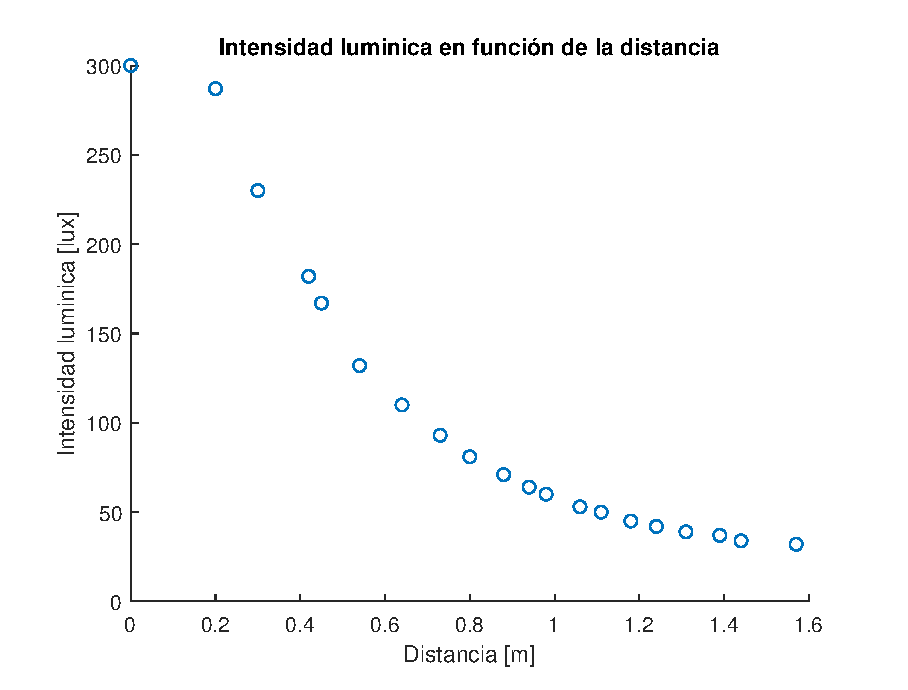
\includegraphics[scale=1.00]{eps/3.1.1.eps}
\caption{Gráfica de intensidad lumínica}
\label{practica31}
\end{figure}

La figura \ref{practica31} sugiere un modelo no lineal, así que se aplicara el
método de logaritmos.

La función tiene la forma general:

\begin{equation}
    y = a x^b
\end{equation}

Aplicando logaritmos a ambos lados de la ecuación, obtenemos:

\begin{equation*}
    \log y = \log a + b \log x
\end{equation*}

Haciendo los siguientes cambios de variables:

\begin{equation*}
    Y' = \log y
\end{equation*}
\begin{equation*}
    A = \log a
\end{equation*}
\begin{equation*}
    B = b
\end{equation*}
\begin{equation*}
    X' = \log x
\end{equation*}

Se obtiene:

\begin{equation*}
    Y' = A + B X'
\end{equation*}

\begin{center}
\begin{tabular}{|c|>{\centering}m{2.8cm}<{\centering}
                  |>{\centering}m{2.8cm}<{\centering}|}
\hline
$i$ & $\log(x_i)$ & $\log(I_i)$ \tabularnewline \hline
  1 & -       & -      \tabularnewline \hline
  2 & -1.6094 & 5.6595 \tabularnewline \hline
  3 & -1.2040 & 5.4381 \tabularnewline \hline
  4 & -0.8675 & 5.2040 \tabularnewline \hline
  5 & -0.7985 & 5.1180 \tabularnewline \hline
  6 & -0.6162 & 4.8828 \tabularnewline \hline
  7 & -0.4463 & 4.7005 \tabularnewline \hline
  8 & -0.3147 & 4.5326 \tabularnewline \hline
  9 & -0.2231 & 4.3944 \tabularnewline \hline
 10 & -0.1278 & 4.2627 \tabularnewline \hline
 11 & -0.0619 & 4.1589 \tabularnewline \hline
 12 & -0.0202 & 4.0943 \tabularnewline \hline
 13 &  0.0583 & 3.9703 \tabularnewline \hline
 14 &  0.1044 & 3.9120 \tabularnewline \hline
 15 &  0.1655 & 3.8067 \tabularnewline \hline
 16 &  0.2151 & 3.7377 \tabularnewline \hline
 17 &  0.2700 & 3.6636 \tabularnewline \hline
 18 &  0.3293 & 3.6109 \tabularnewline \hline
 19 &  0.3646 & 3.5264 \tabularnewline \hline
 20 &  0.4511 & 3.4657 \tabularnewline \hline
\end{tabular}
\end{center}

La gráfica de los datos con el cambio de variable logarítmica pueden verse en la
figura \ref{practica31_2}.

\begin{figure}[!h]
\centering
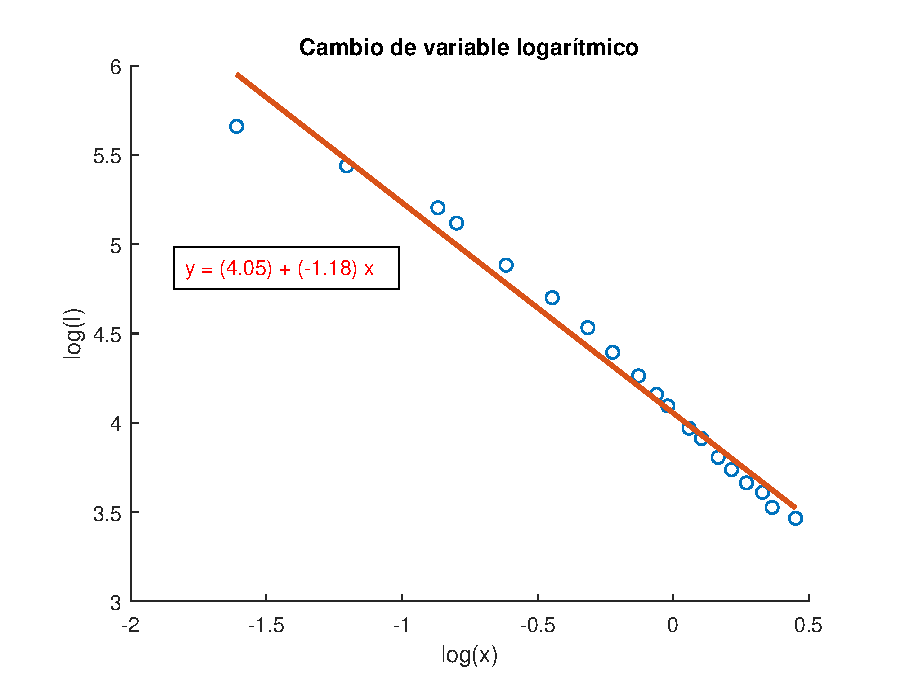
\includegraphics[scale=1.00]{eps/3.1.2.eps}
\caption{Gráfica linealizada por el método de logaritmos}
\label{practica31_2}
\end{figure}

La ecuación de la recta es:

\begin{equation}
    Y = 4.05 - 1.18 x
\end{equation}

A partir de los parámetros de recta $A$ y $B$, calculamos los parámetros $a$ y
$b$, de la curva potencial original:

\begin{equation*}
    a = antilog(A) = antilog(4.05) = 11220.18
\end{equation*}
\begin{equation*}
    b = B = -1.18
\end{equation*}

La ecuación de la curva resultante es:

\begin{equation}
    y = 11220.18 x^{-1.18}
\end{equation}

\subsubsection{Memoria de calculo}

\begin{alltt}
\footnotesize
\input{m/3.1.2.m}
\normalsize
\end{alltt}

Considerando que el exponente de la ecuación final resultó ser: $-1.18$, se
calculará la ecuación por el método del cambio de variable hiperbólico.

La función tiene la forma general:

\begin{equation}
    y = a x^{-1}
\end{equation}

Haciendo el siguiente cambio de variable:

\begin{equation*}
    Z = x^{-1}
\end{equation*}

\begin{center}
\begin{tabular}{|c|>{\centering}m{2.8cm}<{\centering}
                  |>{\centering}m{2.8cm}<{\centering}|}
\hline
$i$ & $x_i^{-1}$ & $I_i$ \tabularnewline \hline
  1 & -      &  -  \tabularnewline \hline
  2 & 5.0000 & 287 \tabularnewline \hline
  3 & 3.3333 & 230 \tabularnewline \hline
  4 & 2.3810 & 182 \tabularnewline \hline
  5 & 2.2222 & 167 \tabularnewline \hline
  6 & 1.8519 & 132 \tabularnewline \hline
  7 & 1.5625 & 110 \tabularnewline \hline
  8 & 1.3699 &  93 \tabularnewline \hline
  9 & 1.2500 &  81 \tabularnewline \hline
 10 & 1.1364 &  71 \tabularnewline \hline
 11 & 1.0638 &  64 \tabularnewline \hline
 12 & 1.0204 &  60 \tabularnewline \hline
 13 & 0.9434 &  53 \tabularnewline \hline
 14 & 0.9009 &  50 \tabularnewline \hline
 15 & 0.8475 &  45 \tabularnewline \hline
 16 & 0.8065 &  42 \tabularnewline \hline
 17 & 0.7634 &  39 \tabularnewline \hline
 18 & 0.7194 &  37 \tabularnewline \hline
 19 & 0.6944 &  34 \tabularnewline \hline
 20 & 0.6369 &  32 \tabularnewline \hline
\end{tabular}
\end{center}

La gráfica de los datos con el cambio de variable hiperbólica pueden verse en la
figura \ref{practica31_3}.

\begin{figure}[!h]
\centering
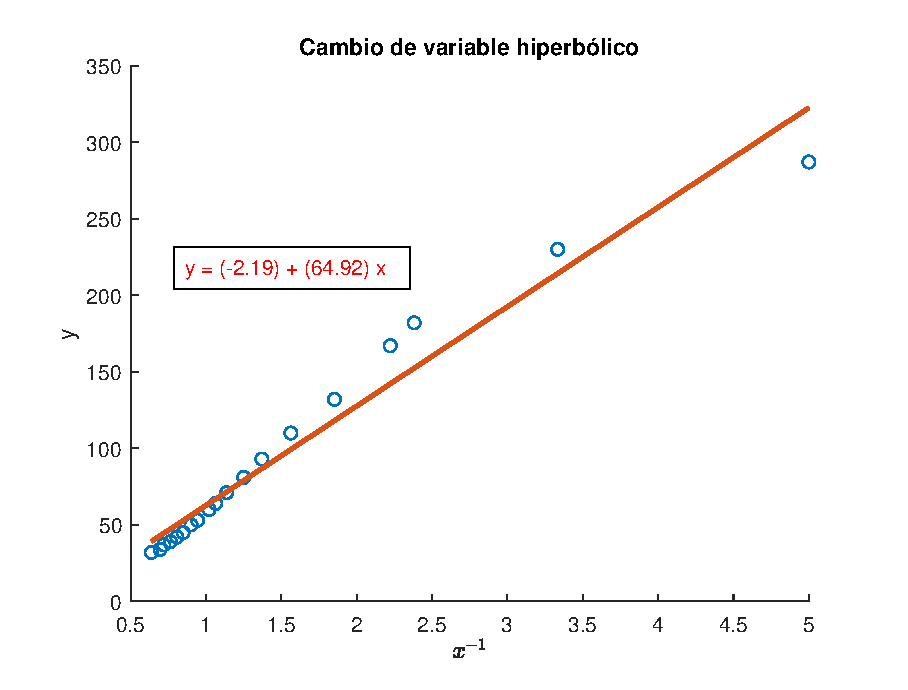
\includegraphics[scale=1.00]{eps/3.1.3.eps}
\caption{Gráfica linealizada por el método de cambio de variable}
\label{practica31_3}
\end{figure}

La ecuación de la recta es:

\begin{equation}
    Y = -2.19 + 64.92 Z
\end{equation}

La ecuación de la curva resultante es:

\begin{equation}
    y = -2.19 + \frac{64.92}{x}
\end{equation}

\subsubsection{Memoria de calculo}

\begin{alltt}
\footnotesize
\input{m/3.2.2.m}
\normalsize
\end{alltt}

\subsection{Presión vs profundidad}
\begin{figure}[!h]
\centering
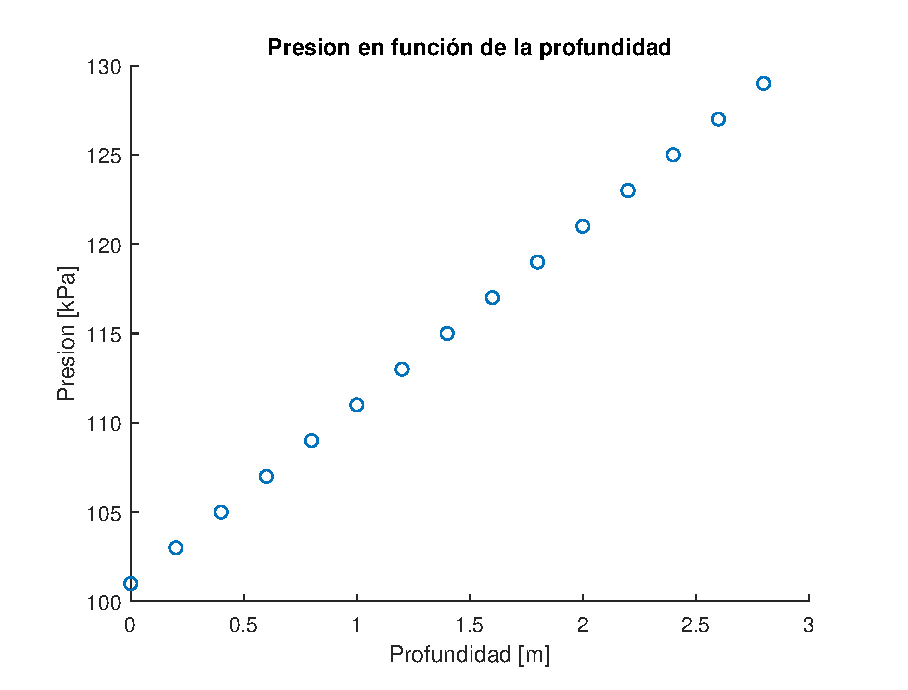
\includegraphics[scale=1.00]{eps/3.2.1.eps}
\caption{Gráfica de presión vs profundidad}
\label{practica32}
\end{figure}

La figura \ref{practica32} sugiere un modelo lineal, así que se calculará la
ecuación de la recta.

La función tiene la forma general:

\begin{equation}
    y = A + B x
\end{equation}

\begin{figure}[!h]
\centering
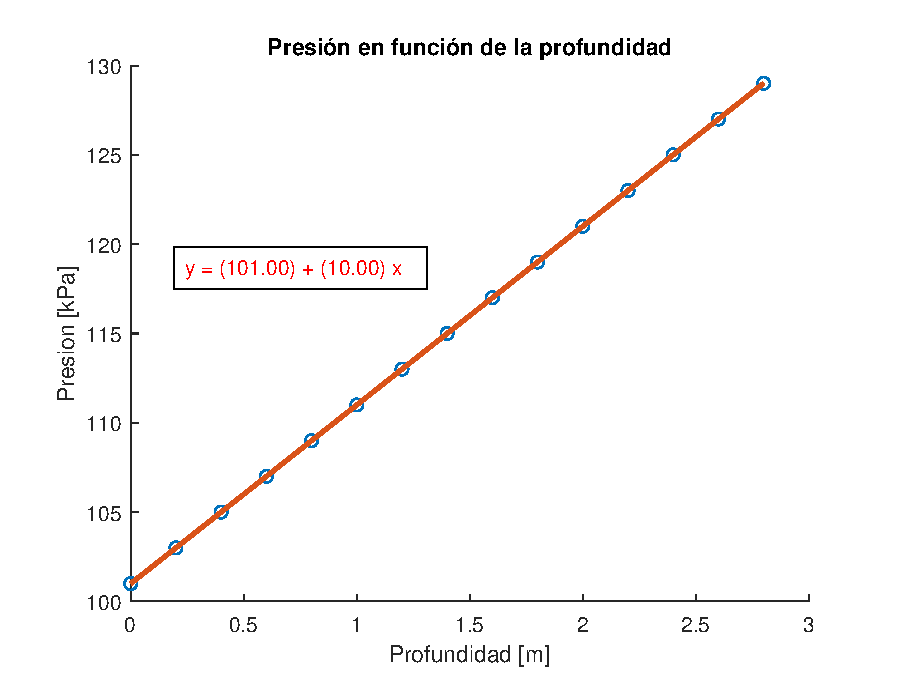
\includegraphics[scale=1.00]{eps/3.2.2.eps}
\caption{Ecuación de presión vs profundidad}
\label{practica32_2}
\end{figure}

La ecuación de la recta es:

\begin{equation}
    y = 101 + 10 x
\end{equation}

\subsubsection{Memoria de calculo}

\begin{alltt}
\footnotesize
\input{m/3.3.2.m}
\normalsize
\end{alltt}

\subsection{Resistencia vs temperatura}
\begin{figure}[!h]
\centering
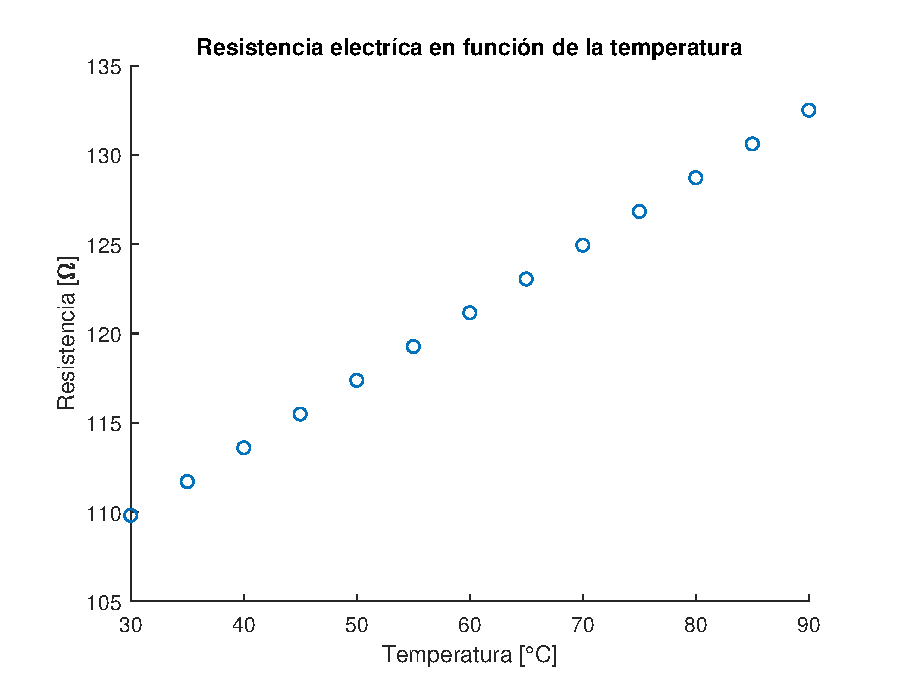
\includegraphics[scale=1.00]{eps/3.3.1.eps}
\caption{Gráfica de resistencia vs temperatura}
\label{practica33}
\end{figure}

La figura \ref{practica33} sugiere un modelo lineal, así que se calculará la
ecuación de la recta.

La función tiene la forma general:

\begin{equation}
    y = A + B x
\end{equation}

\begin{figure}[!h]
\centering
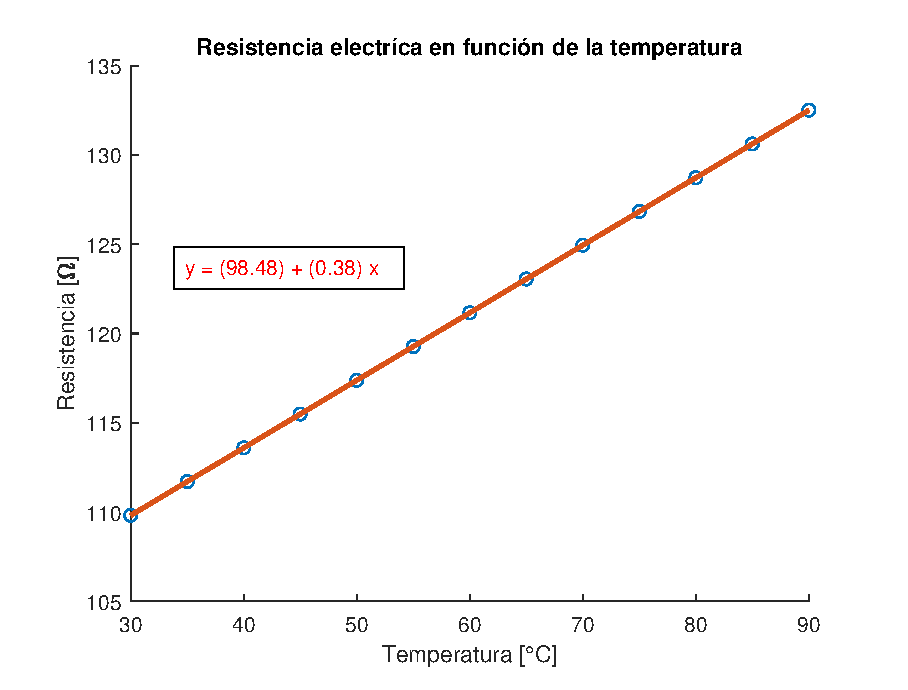
\includegraphics[scale=1.00]{eps/3.3.2.eps}
\caption{Ecuación de la resistencia vs temperatura}
\label{practica33_2}
\end{figure}

La ecuación de la recta es:

\begin{equation}
    y = 98.48 + 0.38 x
\end{equation}

\footnotesize
\begin{verbatim}
% leer datos previamente formateados
table = readtable('./practica33.csv')

% calcular la ecuacion de la recta
p = polyfit(table.Var1, table.Var2, 1)
v = polyval(p, table.Var1)

% personalizar grafica
title('Resistencia eléctrica en función de la temperatura')
xlabel('Temperatura [°C]')
ylabel('Resistencia [\Omega]')

% texto y grafica de ecuacion
caption = sprintf('y = (%.2f) + (%.2f) x', p(2), p(1))
dim = [.18 .35 0 .3]
a = annotation('textbox',dim,'String',caption,'FitBoxToText','on')
a.Color = 'red'
a.FontSize = 10

% graficar puntos y lineas
hold on
plot(table.Var1, table.Var2, 'o')
plot(table.Var1, v, 'LineWidth', 2)
hold off
\end{verbatim}
\normalsize

\subsection{Péndulo}
\begin{figure}[!h]
\centering
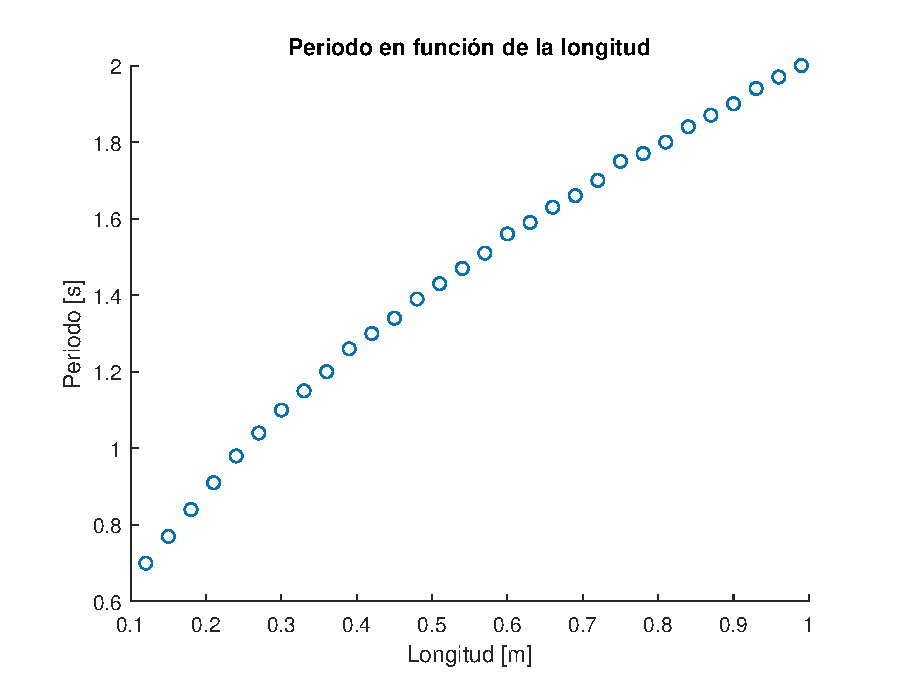
\includegraphics[scale=1.00]{eps/3.4.1.eps}
\caption{Gráfica del péndulo}
\label{practica34}
\end{figure}

La figura \ref{practica34} sugiere un modelo no lineal, así que se aplicara el
método de logaritmos.

La función tiene la forma general:

\begin{equation}
    y = a x^b
\end{equation}

Aplicando logaritmos a ambos lados de la ecuación, obtenemos:

\begin{equation*}
    \log y = \log a + b \log x
\end{equation*}

Haciendo los siguientes cambios de variables:

\begin{equation*}
    Y' = \log y
\end{equation*}
\begin{equation*}
    A = \log a
\end{equation*}
\begin{equation*}
    B = b
\end{equation*}
\begin{equation*}
    X' = \log x
\end{equation*}

Se obtiene:

\begin{equation*}
    Y' = A + B X'
\end{equation*}

\begin{center}
\begin{tabular}{|c|>{\centering}m{2.8cm}<{\centering}
                  |>{\centering}m{2.8cm}<{\centering}|}
\hline
$i$ & $\log(L_i)$ & $\log(T_i)$ \tabularnewline \hline
  1 &  -      &  -      \tabularnewline \hline
  2 & -1.8971 & -0.2614 \tabularnewline \hline
  3 & -1.7148 & -0.1744 \tabularnewline \hline
  4 & -1.5606 & -0.0943 \tabularnewline \hline
  5 & -1.4271 & -0.0202 \tabularnewline \hline
  6 & -1.3093 &  0.0392 \tabularnewline \hline
  7 & -1.2040 &  0.0953 \tabularnewline \hline
  8 & -1.1087 &  0.1398 \tabularnewline \hline
  9 & -1.0217 &  0.1823 \tabularnewline \hline
 10 & -0.9416 &  0.2311 \tabularnewline \hline
 11 & -0.8675 &  0.2624 \tabularnewline \hline
 12 & -0.7985 &  0.2927 \tabularnewline \hline
 13 & -0.7340 &  0.3293 \tabularnewline \hline
 14 & -0.6733 &  0.3577 \tabularnewline \hline
 15 & -0.6162 &  0.3853 \tabularnewline \hline
 16 & -0.5621 &  0.4121 \tabularnewline \hline
 17 & -0.5108 &  0.4447 \tabularnewline \hline
 18 & -0.4620 &  0.4637 \tabularnewline \hline
 19 & -0.4155 &  0.4886 \tabularnewline \hline
 20 & -0.3711 &  0.5068 \tabularnewline \hline
 21 & -0.3285 &  0.5306 \tabularnewline \hline
 22 & -0.2877 &  0.5596 \tabularnewline \hline
 23 & -0.2485 &  0.5710 \tabularnewline \hline
 24 & -0.2107 &  0.5878 \tabularnewline \hline
 25 & -0.1744 &  0.6098 \tabularnewline \hline
 26 & -0.1393 &  0.6259 \tabularnewline \hline
 27 & -0.1054 &  0.6419 \tabularnewline \hline
 28 & -0.0726 &  0.6627 \tabularnewline \hline
 29 & -0.0408 &  0.6780 \tabularnewline \hline
 30 & -0.0101 &  0.6931 \tabularnewline \hline
\end{tabular}
\end{center}

La gráfica de los datos con el cambio de variable logarítmica pueden verse en la
figura \ref{practica34_2}.

\begin{figure}[!h]
\centering
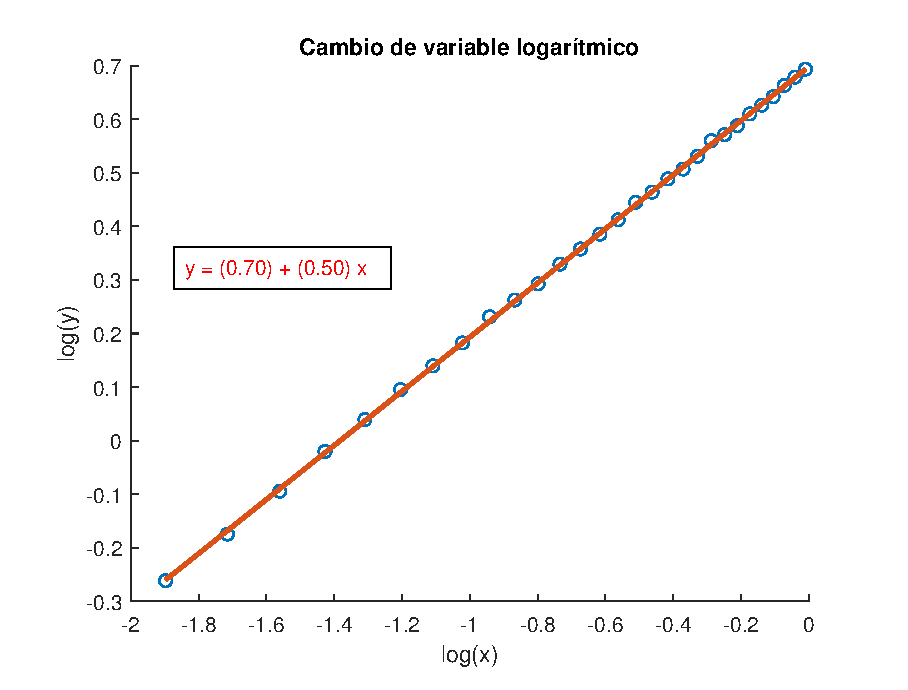
\includegraphics[scale=1.00]{eps/3.4.2.eps}
\caption{Gráfica linealizada por el método de logaritmos}
\label{practica34_2}
\end{figure}

La ecuación de la recta es:

\begin{equation}
    Y = 0.70 + 0.50 x
\end{equation}

A partir de los parámetros de recta $A$ y $B$, calculamos los parámetros $a$ y
$b$, de la curva potencial original:

\begin{equation*}
    a = antilog(A) = antilog(0.70) = 5.0119
\end{equation*}
\begin{equation*}
    b = B = 0.50
\end{equation*}

La ecuación de la curva resultante es:

\begin{equation}
    y = 5.0119 \sqrt{x}
\end{equation}

\subsubsection{Memoria de calculo}

\begin{alltt}
\footnotesize
\input{m/3.4.2.m}
\normalsize
\end{alltt}

Considerando que el exponente de la ecuación final resultó ser: $0.5$, se
calculará la ecuación por el método del cambio de variable.

La función tiene la forma general:

\begin{equation}
    y = a \sqrt{x}
\end{equation}

Haciendo el siguiente cambio de variable:

\begin{equation*}
    Z = \sqrt{x}
\end{equation*}

\begin{center}
\begin{tabular}{|c|>{\centering}m{2.8cm}<{\centering}
                  |>{\centering}m{2.8cm}<{\centering}|}
\hline
$i$ & $\sqrt{T_i}$ & $L_i$ \tabularnewline \hline
  1 & -      & -      \tabularnewline \hline
  2 & 0.3873 & 0.7700 \tabularnewline \hline
  3 & 0.4243 & 0.8400 \tabularnewline \hline
  4 & 0.4583 & 0.9100 \tabularnewline \hline
  5 & 0.4899 & 0.9800 \tabularnewline \hline
  6 & 0.5196 & 1.0400 \tabularnewline \hline
  7 & 0.5477 & 1.1000 \tabularnewline \hline
  8 & 0.5745 & 1.1500 \tabularnewline \hline
  9 & 0.6000 & 1.2000 \tabularnewline \hline
 10 & 0.6245 & 1.2600 \tabularnewline \hline
 11 & 0.6481 & 1.3000 \tabularnewline \hline
 12 & 0.6708 & 1.3400 \tabularnewline \hline
 13 & 0.6928 & 1.3900 \tabularnewline \hline
 14 & 0.7141 & 1.4300 \tabularnewline \hline
 15 & 0.7348 & 1.4700 \tabularnewline \hline
 16 & 0.7550 & 1.5100 \tabularnewline \hline
 17 & 0.7746 & 1.5600 \tabularnewline \hline
 18 & 0.7937 & 1.5900 \tabularnewline \hline
 19 & 0.8124 & 1.6300 \tabularnewline \hline
 20 & 0.8307 & 1.6600 \tabularnewline \hline
 21 & 0.8485 & 1.7000 \tabularnewline \hline
 22 & 0.8660 & 1.7500 \tabularnewline \hline
 23 & 0.8832 & 1.7700 \tabularnewline \hline
 24 & 0.9000 & 1.8000 \tabularnewline \hline
 25 & 0.9165 & 1.8400 \tabularnewline \hline
 26 & 0.9327 & 1.8700 \tabularnewline \hline
 27 & 0.9487 & 1.9000 \tabularnewline \hline
 28 & 0.9644 & 1.9400 \tabularnewline \hline
 29 & 0.9798 & 1.9700 \tabularnewline \hline
 30 & 0.9950 & 2.0000 \tabularnewline \hline
\end{tabular}
\end{center}

La gráfica de los datos con el cambio de variable puede verse en la figura
\ref{practica34_3}.

\begin{figure}[!h]
\centering
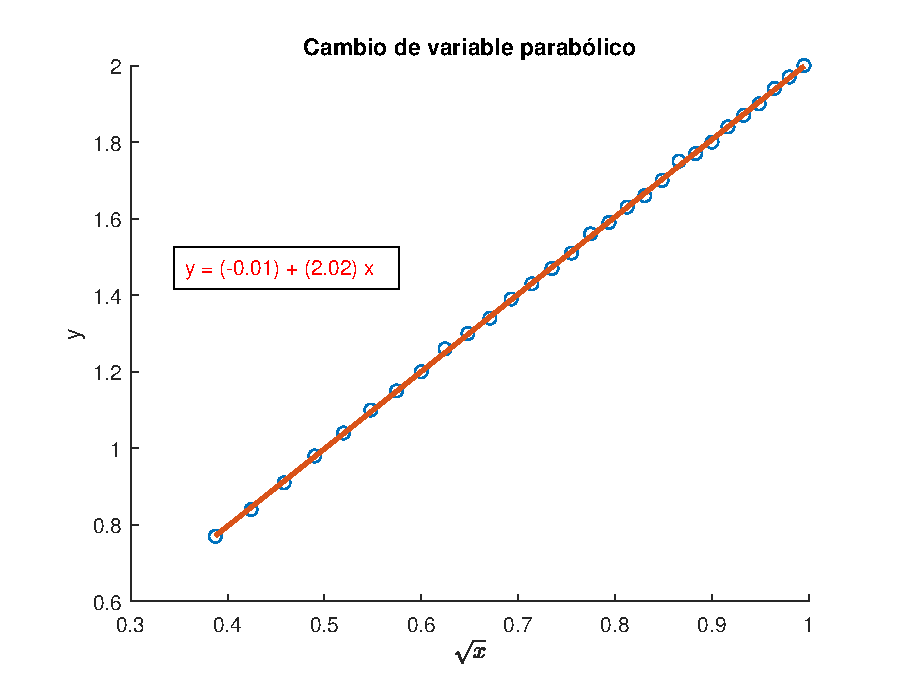
\includegraphics[scale=1.00]{eps/3.4.3.eps}
\caption{Gráfica linealizada por el método de cambio de variable}
\label{practica34_3}
\end{figure}

La ecuación de la recta es:

\begin{equation}
    y = -0.01 + 2.02 Z
\end{equation}

La ecuación de la curva resultante es:

\begin{equation}
    y = -0.01 + 2.02 \sqrt{x}
\end{equation}

\footnotesize
\begin{verbatim}
% leer datos previamente formateados
table = readtable('./practica34.csv')

% cambio de variable
X = table.Var1(2:end).^(0.5)
Y = table.Var2(2:end)

% calcular la ecuacion de la recta
p = polyfit(X, Y, 1)
v = polyval(p, X)

% personalizar grafica
title('Cambio de variable parabólico')
xlabel('$\sqrt{x}$','interpreter','latex')
ylabel('y')

% texto y grafica de ecuacion
caption = sprintf('y = (%.2f) + (%.2f) x', p(2), p(1))
dim = [.18 .35 0 .3]
a = annotation('textbox',dim,'String',caption,'FitBoxToText','on')
a.Color = 'red'
a.FontSize = 10

% graficar puntos y lineas
hold on
plot(X, Y, 'o')
plot(X, v, 'LineWidth', 2)
hold off
\end{verbatim}
\normalsize

\section{Conclusiones}
Se aprendió a graficar diferentes relaciones entre variables sean lineales o
no lineales, como también calcular la ecuación que rige su comportamiento.

\subsection{Resultados obtenidos}

\begin{center}
\begin{tabular}{|c|c|}
\hline
\multicolumn{2}{|c|}{\textbf{Intensidad lumínica}} \\
\multicolumn{2}{|c|}{$y = 11220.18 x^{-1.18}$} \\
\multicolumn{2}{|c|}{$y = -2.19 + 64.92 x^{-1}$} \\
\hline
\multicolumn{2}{|c|}{\textbf{Presión vs profundidad}} \\
\multicolumn{2}{|c|}{$y = 101 + 10 x$} \\
\hline
\multicolumn{2}{|c|}{\textbf{Resistencia vs temperatura}} \\
\multicolumn{2}{|c|}{$y = 98.48 + 0.38 x$} \\
\hline
\multicolumn{2}{|c|}{\textbf{Péndulo}} \\
\multicolumn{2}{|c|}{$y = 5.0119 \sqrt{x}$} \\
\multicolumn{2}{|c|}{$y = -0.01 + 2.02 \sqrt{x}$} \\
\hline
\end{tabular}
\end{center}

\end{document}
